\documentclass[crop,tikz]{standalone}% 'crop' is the default for v1.0, before it was 'preview'
\usepackage{tikz}
\usetikzlibrary{positioning,arrows,calc,shapes}
\begin{document}
\def\layersep{2.0cm}

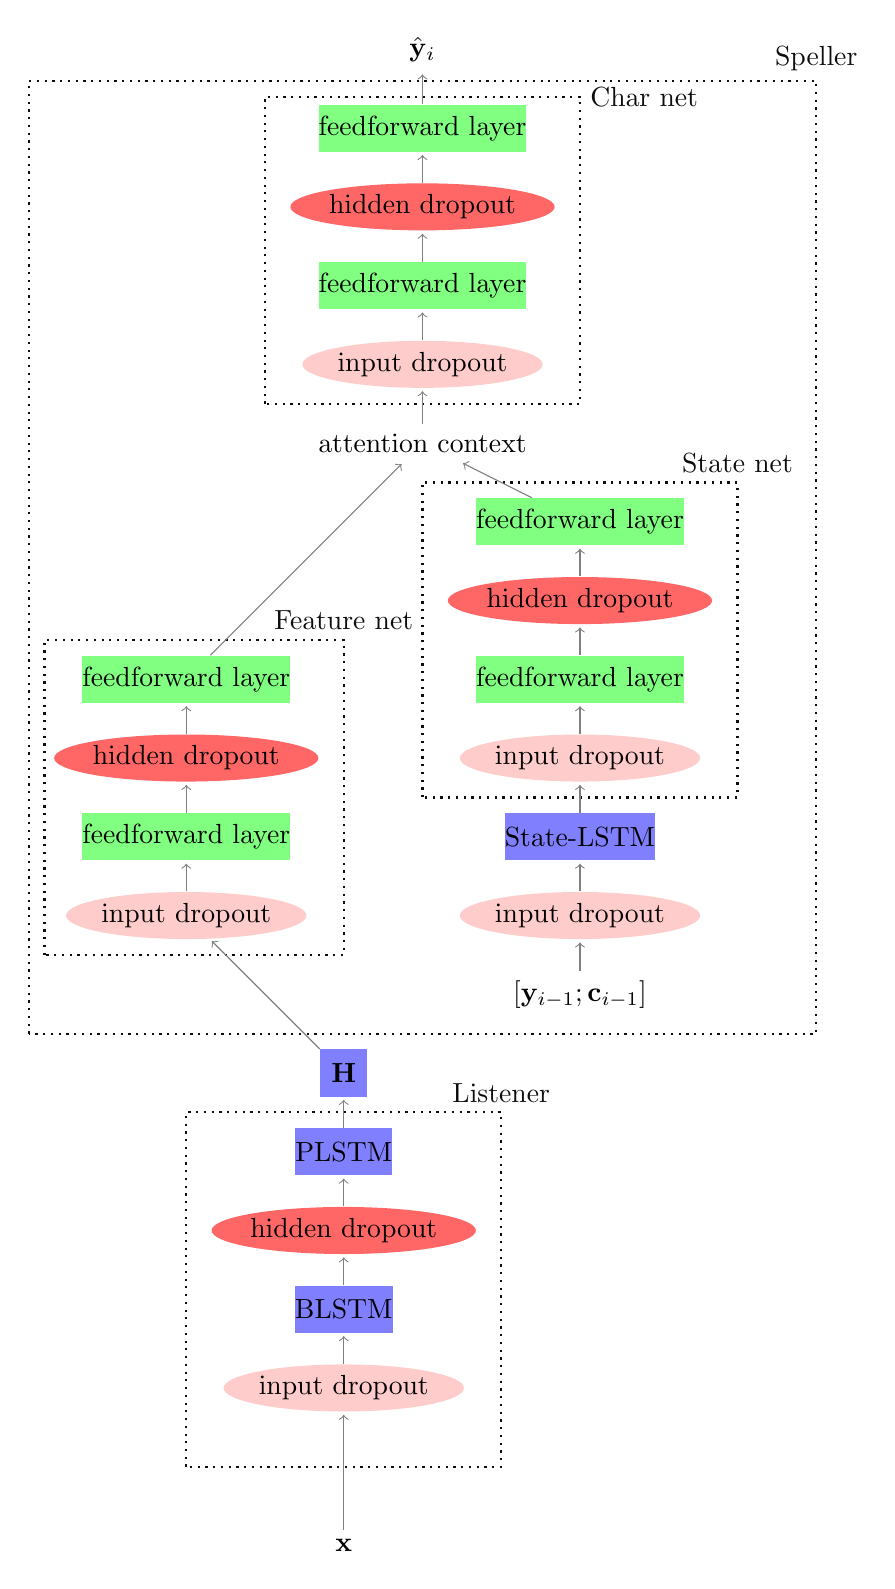
\begin{tikzpicture}[shorten >=1pt,->,draw=black!50, node distance=\layersep,transform shape,rotate=00]  %<-- rotate the NN
	\tikzstyle{every pin edge}=[<-,shorten <=1pt]
	\tikzstyle{dropout}=[ellipse,fill=black!25,minimum size=17pt,inner sep=0pt]
	\tikzstyle{inDrop}=[dropout, fill=red!20];
	\tikzstyle{hiddenDrop}=[dropout, fill=red!60];
		
	\tikzstyle{layer}=[rectangle,fill=black!25,minimum size=17pt,inner sep=0pt]
	\tikzstyle{fflayer}=[layer, fill=green!50];
	\tikzstyle{rnnlayer}=[layer, fill=blue!50];
	
	%listener
	\draw[black!95,thick,dotted] (0,1)  rectangle (4,5.5) node[above]{Listener};
	\node (x) at (2,0) {$\mathbf{x}$};
	\node[inDrop] (inputDrop) at (2,2) {input dropout};
	\node[rnnlayer] (listenerBLSTM) at (2,3) {BLSTM};
	\node[hiddenDrop] (listenDrop) at (2,4) {hidden dropout};
	\node[rnnlayer] (listenerPLSTM) at (2,5) {PLSTM};
	\draw[->] (x) -- (inputDrop);
	\draw[->] (inputDrop) -- (listenerBLSTM);
	\draw[->] (listenerBLSTM) -- (listenDrop);
	\draw[->] (listenDrop) -- (listenerPLSTM);

	\node[rnnlayer] (H) at (2,6) {$\mathbf{H}$};
	\draw[->] (listenerPLSTM) -- (H);
				
	%feature net
	\draw[black!95,thick,dotted] (-1.8,7.5)  rectangle (2,11.5) node[above]{Feature net};
	\node[inDrop] (featDrop) at (0,8) {input dropout};
	\node[fflayer] (featFF1) at (0,9) {feedforward layer};
	\node[hiddenDrop] (feathiddenDrop) at (0,10) {hidden dropout};
	\node[fflayer] (featFF2) at (0,11) {feedforward layer};
	\draw[->] (H) -- (featDrop);
	\draw[->] (featDrop) -- (featFF1);
	\draw[->] (featFF1) -- (feathiddenDrop);
	\draw[->] (feathiddenDrop) -- (featFF2);
		

	%as cell	
	\draw[black!95,thick,dotted] (-2,6.5)  rectangle (8,18.6) node[above]{Speller};
	\node (stateIn) at (5,7) {$[\mathbf{y}_{i-1}; \mathbf{c}_{i-1}]$};
	\node[inDrop] (stateInDrop) at (5,8) {input dropout};
	\node[rnnlayer] (asLSTM) at (5,9) {State-LSTM};
	\draw[->] (stateIn) -- (stateInDrop);
	\draw[->] (stateInDrop) -- (asLSTM);
		
		%state net
		\draw[black!95,thick,dotted] (3.0,9.5)  rectangle (7,13.5) node[above]{State net};
		\node[inDrop] (featInDrop) at (5,10) {input dropout};
		\node[fflayer] (stateFF1) at (5,11) {feedforward layer};
		\node[hiddenDrop] (stateHiddenDrop) at (5,12) {hidden dropout};
		\node[fflayer] (stateFF2) at (5,13) {feedforward layer};
		\draw[->] (asLSTM) -- (featInDrop);
		\draw[->] (featInDrop) -- (stateFF1);
		\draw[->] (stateFF1) -- (stateHiddenDrop);
		\draw[->] (stateHiddenDrop) -- (stateFF2);
	
		%context
		\node (attentionContext) at (3,14) {attention context};
		\draw[->] (stateFF2) -- (attentionContext);
		\draw[->] (featFF2) -- (attentionContext);
		
		%char net
		\draw[black!95,thick,dotted] (1.0,14.5)  rectangle (5,18.4) node[right]{Char net};
		\node[inDrop] (charDrop) at (3,15) {input dropout};
		\node[fflayer] (charFF1) at (3,16) {feedforward layer};
		\node[hiddenDrop] (charHiddenDrop) at (3,17) {hidden dropout};
		\node[fflayer] (charFF2) at (3,18) {feedforward layer};
		\draw[->] (attentionContext) -- (charDrop);
		\draw[->] (charDrop) -- (charFF1);
		\draw[->] (charFF1) -- (charHiddenDrop);
		\draw[->] (charHiddenDrop) -- (charFF2);
	\node (char) at (3,19) {$\hat{\mathbf{y}}_i$};
	\draw[->] (charFF2) -- (char);

\end{tikzpicture}
% End of code
\end{document}
